\documentclass[
11pt, % Set the default font size, options include: 8pt, 9pt, 10pt, 11pt, 12pt, 14pt, 17pt, 20pt
%t, % Uncomment to vertically align all slide content to the top of the slide, rather than the default centered
%aspectratio=169, % Uncomment to set the aspect ratio to a 16:9 ratio which matches the aspect ratio of 1080p and 4K screens and projectors
]{beamer}

\graphicspath{{Images/}{./}} % Specifies where to look for included images (trailing slash required)

\usepackage{todonotes}
\usepackage{graphicx}
\usepackage{xcolor}
\usepackage{subfig}
%%\usepackage[noend]{algpseudocode}

%
%\usepackage{algorithm}
%\usepackage{algorithmic}
\usepackage{algorithm}
\usepackage{algpseudocode}
\usepackage{blkarray}
\usepackage{amsmath}
\usepackage{xspace}
\usepackage{float}


\usepackage{tikz}
\usetikzlibrary{matrix, decorations, patterns, positioning, shapes, calc, intersections, arrows, fit}

\usetikzlibrary{patterns}
\usetikzlibrary{fit,calc,positioning,decorations.pathreplacing,matrix,3d, hobby}

\usepackage{booktabs} % Allows the use of \toprule, \midrule and \bottomrule for better rules in tables
\usepackage{bm}
\usepackage{multirow}

\newcommand{\brown}[1]{{\color{brown} #1 }}

%% Colors from https://latexcolor.com/
\definecolor{pastelviolet}{rgb}{0.8, 0.6, 0.79}
\definecolor{babyblueeyes}{rgb}{0.63, 0.79, 0.95}
\definecolor{pastelyellow}{rgb}{0.99, 0.99, 0.59}
\definecolor{pastelgreen}{rgb}{0.47, 0.87, 0.47}
\definecolor{pastelred}{rgb}{1.0, 0.41, 0.38}
\colorlet{patternblue}{blue!60}


\colorlet{darkred}{red!80!black}
\colorlet{darkblue}{blue!80!black}
\newcommand<>{\darkred}[1]{{\color{darkred}{#1}}}
\newcommand<>{\darkblue}[1]{{\color#2{blue!50!black!100}{#1}}}

\newcommand{\A}{\mathbf{A}}
\newcommand{\B}{\mathbf{B}}
\newcommand{\CC}{\mathbf{C}}
%\newcommand{\Real}{\mathbb{R}}
\newcommand{\vc}[1]{\bm{#1}}

\usetheme{Madrid}

%\newcommand{\Tra}{{\sf T}} 


%\newcommand{\Ms}[2]{\mathbf{#1}^{(#2)}} 
%\newcommand{\M}[1]{\mathbf{#1}} 
%\newcommand{\Mb}[2]{\mathbf{#1}_{#2}} 
%\newcommand{\Mbs}[3]{\mathbf{#1}_{#2}^{(#3)}} 

%\usepackage{enumitem}

%% ------------------------------------------------------------
%% PACKAGES
%% ------------------------------------------------------------

%% For \circledast
\usepackage{amssymb,amsfonts,amsmath}

%% For \mathscr
\usepackage[mathscr]{eucal}

%% For \llbracket and \rrbracket, \varoast, \varoslash
\usepackage{stmaryrd}

%% For \boldsymbol
\usepackage{amsbsy}

%% For \bm (bold math)
\usepackage{bm}

%% For \set, \Set
\usepackage{braket}

%% ------------------------------------------------------------
%% MACROS
%% ------------------------------------------------------------


%% --- Extras ---
% Transpose
\newcommand{\Tra}{{\sf T}} 
\newcommand{\parens}[1]{(#1)}
\newcommand{\Parens}[1]{\left(#1\right)}
\newcommand{\dsquare}[1]{\llbracket #1 \rrbracket}
\newcommand{\Dsquare}[1]{\left\llbracket #1 \right\rrbracket}
\newcommand{\curly}[1]{\{ #1 \}}
\newcommand{\Curly}[1]{\left\{ #1 \right\}}
\newcommand{\Real}{\mathbb{R}}
\newcommand{\qtext}[1]{\quad\text{#1}\quad}

%% --- Vectors ---
% vector
\newcommand{\V}[2][]{{\bm{#1\mathbf{\MakeLowercase{#2}}}}} 
% element of vector
\newcommand{\VE}[3][]{#1{\MakeLowercase{#2}}_{#3}} 
% vector in series
\newcommand{\Vn}[3][]{{\bm{#1\mathbf{\MakeLowercase{#2}}}}^{(#3)}} 
% transposed vector in series
\newcommand{\VnTra}[3][]{{\bm{#1\mathbf{\MakeLowercase{#2}}}}^{(#3)\Tra}} 
% element of vector in series
\newcommand{\VnE}[4][]{#1{\MakeLowercase{#2}}^{(#3)}_{#4}} 

%% --- Matrices ---
% matrix
\newcommand{\M}[2][]{{\bm{#1\mathbf{\MakeUppercase{#2}}}}} 
% matrix in series
\newcommand{\Mn}[3][]{{\bm{#1\mathbf{\MakeUppercase{#2}}}}^{(#3)}} 
% transposed matrix in series 
\newcommand{\MnTra}[4][]{{\bm{#1\mathbf{\MakeUppercase{#2}}}}^{(#3)\Tra}} 
% matrix column
\newcommand{\MC}[3][]{\V[#1]{#2}_{#3}} 
% column of matrix in series
\newcommand{\MnC}[4][]{\Vn[#1]{#2}{#3}_{#4}} 
% transposed column of matrix in series
\newcommand{\MnCTra}[4][]{\VnTra[#1]{#2}{#3}_{#4}} 
% matrix element
\newcommand{\ME}[3][]{#1{\MakeLowercase{#2}}_{#3}} 
% element of matrix in series
\newcommand{\MnE}[4][]{#1{\MakeLowercase{#2}}^{(#3)}_{#4}} 

%% --- Tensors ---
% tensor
\newcommand{\T}[2][]{\boldsymbol{#1\mathscr{\MakeUppercase{#2}}}} 
% tensor slide
\newcommand{\TS}[3][]{\M[#1]{#2}_{#3}}
% tensor element
\newcommand{\TE}[3][]{#1{\MakeLowercase{#2}}_{#3}}
% matriczied tensor
\newcommand{\Mz}[3][]{\M[#1]{#2}_{(#3)}}

%% --- Operators ---
% outer product
\newcommand{\Oprod}{\circ} 
% Kronecker product
\newcommand{\Kron}{\otimes} 
% Khatri-Rao product
\newcommand{\Khat}{\odot} 
% Hadamard (elementwise multiply)
\newcommand{\Hada}{\ast} 
\newcommand{\BigHada}{\mathop{\mbox{\fontsize{18}{19}\selectfont $\circledast$}}} 
% Elementwise divide
\newcommand{\Divi}{\varoslash}





%----------------------------------------------------------------------------------------
%	PRESENTATION INFORMATION
%----------------------------------------------------------------------------------------

\title[Tensors]{Introduction to Tensors} % The short title in the optional parameter appears at the bottom of every slide, the full title in the main parameter is only on the title page

%\subtitle{Optional Subtitle} % Presentation subtitle, remove this command if a subtitle isn't required

\author[Suraj Kumar]{Suraj Kumar} % Presenter name(s), the optional parameter can contain a shortened version to appear on the bottom of every slide, while the main parameter will appear on the title slide

\institute[Inria \& ENS Lyon]{Inria \& ENS Lyon \\ \smallskip Email:\textit{suraj.kumar@inria.fr}} % Your institution, the optional parameter can be used for the institution shorthand and will appear on the bottom of every slide after author names, while the required parameter is used on the title slide and can include your email address or additional information on separate lines

\date[CR12]{CR12: September 2023\\ \smallskip\small https://surakuma.github.io/courses/daamtc.html} % Presentation date or conference/meeting name, the optional parameter can contain a shortened version to appear on the bottom of every slide, while the required parameter value is output to the title slide

%----------------------------------------------------------------------------------------

\begin{document}
	
	%----------------------------------------------------------------------------------------
	%	TITLE SLIDE
	%----------------------------------------------------------------------------------------
	
	\begin{frame}
		\titlepage % Output the title slide, automatically created using the text entered in the PRESENTATION INFORMATION block above
	\end{frame}


\begin{frame}{Tensors (multidimensional arrays)}
	\begin{center}
		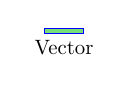
\begin{tikzpicture}[scale=0.125, every node/.style={transform shape}]
		\pgfmathsetmacro{\rectx}{4}
		\pgfmathsetmacro{\recty}{0.5}
		\draw[blue,fill=pastelgreen] (0,0) -- node [below, scale=6, black] {Vector}++(-\rectx,0) -- ++(0,\recty) -- ++(\rectx, 0) -- cycle;
		\end{tikzpicture}$\;$
		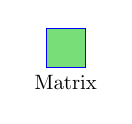
\begin{tikzpicture}[scale=0.125, every node/.style={transform shape}]
		\pgfmathsetmacro{\rectx}{4}
		\pgfmathsetmacro{\recty}{4}
		\draw[blue,fill=pastelgreen] (0,0) -- node [below, scale=6, black] {Matrix}++(-\rectx,0) -- ++(0,\recty) -- ++(\rectx, 0) -- cycle;
		%%\addvmargin{4};
		\end{tikzpicture}$\;$
		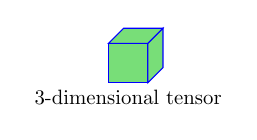
\begin{tikzpicture}[scale=0.125, every node/.style={transform shape}]
		\pgfmathsetmacro{\cubex}{4}
		\pgfmathsetmacro{\cubey}{4}
		\pgfmathsetmacro{\cubez}{4}
		\draw[blue,fill=pastelgreen] (0,0,0) -- ++(-\cubex,0,0) -- ++(0,-\cubey,0) --node [below, scale=6, black] {3-dimensional tensor} ++(\cubex,0,0) -- cycle;
		\draw[blue,fill=pastelgreen] (0,0,0) -- ++(0,0,-\cubez) -- ++(0,-\cubey,0) -- ++(0,0,\cubez) -- cycle;
		\draw[blue,fill=pastelgreen] (0,0,0) -- ++(-\cubex,0,0) -- ++(0,0,-\cubez) -- ++(\cubex,0,0) -- cycle;
		\end{tikzpicture}$\;$
		%%	\end{center}
		%%	\begin{center}	
		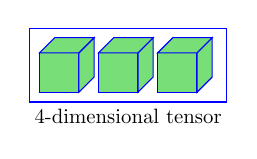
\begin{tikzpicture}[scale=0.125, every node/.style={transform shape}]
		\pgfmathsetmacro{\cubex}{4}
		\pgfmathsetmacro{\cubey}{4}
		\pgfmathsetmacro{\cubez}{4}
		\draw[blue,fill=pastelgreen] (0,0,0) -- ++(-\cubex,0,0) -- ++(0,-\cubey,0) -- ++(\cubex,0,0) -- cycle;
		\draw[blue,fill=pastelgreen] (0,0,0) -- ++(0,0,-\cubez) -- ++(0,-\cubey,0) -- ++(0,0,\cubez) -- cycle;
		\draw[blue,fill=pastelgreen] (0,0,0) -- ++(-\cubex,0,0) -- ++(0,0,-\cubez) -- ++(\cubex,0,0) -- cycle;
		
		\draw[blue,fill=pastelgreen] (\cubex +2,0,0) -- ++(-\cubex,0,0) -- ++(0,-\cubey,0) -- ++(\cubex,0,0) -- cycle;
		\draw[blue,fill=pastelgreen] (\cubex +2,0,0) -- ++(0,0,-\cubez) -- ++(0,-\cubey,0) -- ++(0,0,\cubez) -- cycle;
		\draw[blue,fill=pastelgreen] (\cubex +2,0,0) -- ++(-\cubex,0,0) -- ++(0,0,-\cubez) -- ++(\cubex,0,0) -- cycle;
		
		\draw[blue,fill=pastelgreen] (\cubex +2 + \cubex +2,0,0) -- ++(-\cubex,0,0) -- ++(0,-\cubey,0) -- ++(\cubex,0,0) -- cycle;
		\draw[blue,fill=pastelgreen] (\cubex +2 + \cubex +2,0,0) -- ++(0,0,-\cubez) -- ++(0,-\cubey,0) -- ++(0,0,\cubez) -- cycle;
		\draw[blue,fill=pastelgreen] (\cubex +2 + \cubex +2,0,0) -- ++(-\cubex,0,0) -- ++(0,0,-\cubez) -- ++(\cubex,0,0) -- cycle;
		
		\draw[blue, fill=none] (-\cubex -1, 2.5, 0) -- ++(0, -\cubey -3.5, 0) --node [below, scale=6, black] {4-dimensional tensor} ++(\cubex +2 + \cubex +2 + \cubex + \cubex,0,0) -- ++(0, \cubey +3.5, 0) -- cycle; 
		
		%%\node [scale=2] at (0, -8) {$hello$};
		\end{tikzpicture}
	\end{center}
	
	\vfill
	\small
	\begin{itemize}
		\item \textbf{Neuroscience}: measure of calcium fluorescence in a particular pixel during a time step of a single trial (Pixel $\times$ Time $\times$ Trial)
		\vfill
		\item \textbf{Combustion simulation}: value of a variable in a spatial grid during a time step (Grid length $\times$ Grid width $\times$ Grid height $\times$ Variable $\times$ Time)
		\vfill
		\item \textbf{Media}: rating of a movie by a user during a time slice (User $\times$ Movie $\times$ Time)
		\vfill
		\item \textbf{Molecular/quantum simulations}: interaction of electrons in $d$ orbitals with a $4^d$ tensor
		
%		%%		\item \textbf{Transportation}: Pickup $\times$ Dropoff $\times$ Time
%		\item  
%		\item \textbf{Ecommerce}: User x Product x Time
%		\item \textbf{Social-Network}: Person x Person x Time x Type
%		%%		\item[$\textcolor{blue}{\bullet}$] \textbf{Social-Network}: Person x Person x Time x Type
	\end{itemize}
\vfill
Notation convention: Matrix $A$, tensor $\T{A}$	
\end{frame}

\section{Tensor notations and some definitions}
	\begin{frame}{Table of Contents}		
	\tableofcontents[currentsection,hideallsubsections] % Output the table of contents (all sections on one slide)		
	\end{frame}


\begin{frame}{Tensor notations (following [Kolda and Bader, 2009])}
	\small
Let $\T{A}$ be a $d$-dimensional tensor of size $n_1\times n_2\times\cdots \times n_d$, $\T{A} \in \mathbb{R}^{n_1\times n_2\times \cdots \times n_d}$.
\begin{itemize}
	\item $d=1$ , first order tensors: vectors
	\item $d=2$, second order tensors: matrices
\end{itemize}
\vfill
The element of $\T{A}$ is denoted as $\T{A}(i_1,i_2,\ldots,i_d)$.
\vfill
\begin{minipage}{0.45\linewidth}
	\begin{itemize}
		\item Fibers: defined by fixing all indices except one
	\end{itemize}
		\vspace*{-0.525cm}
		\begin{center}
		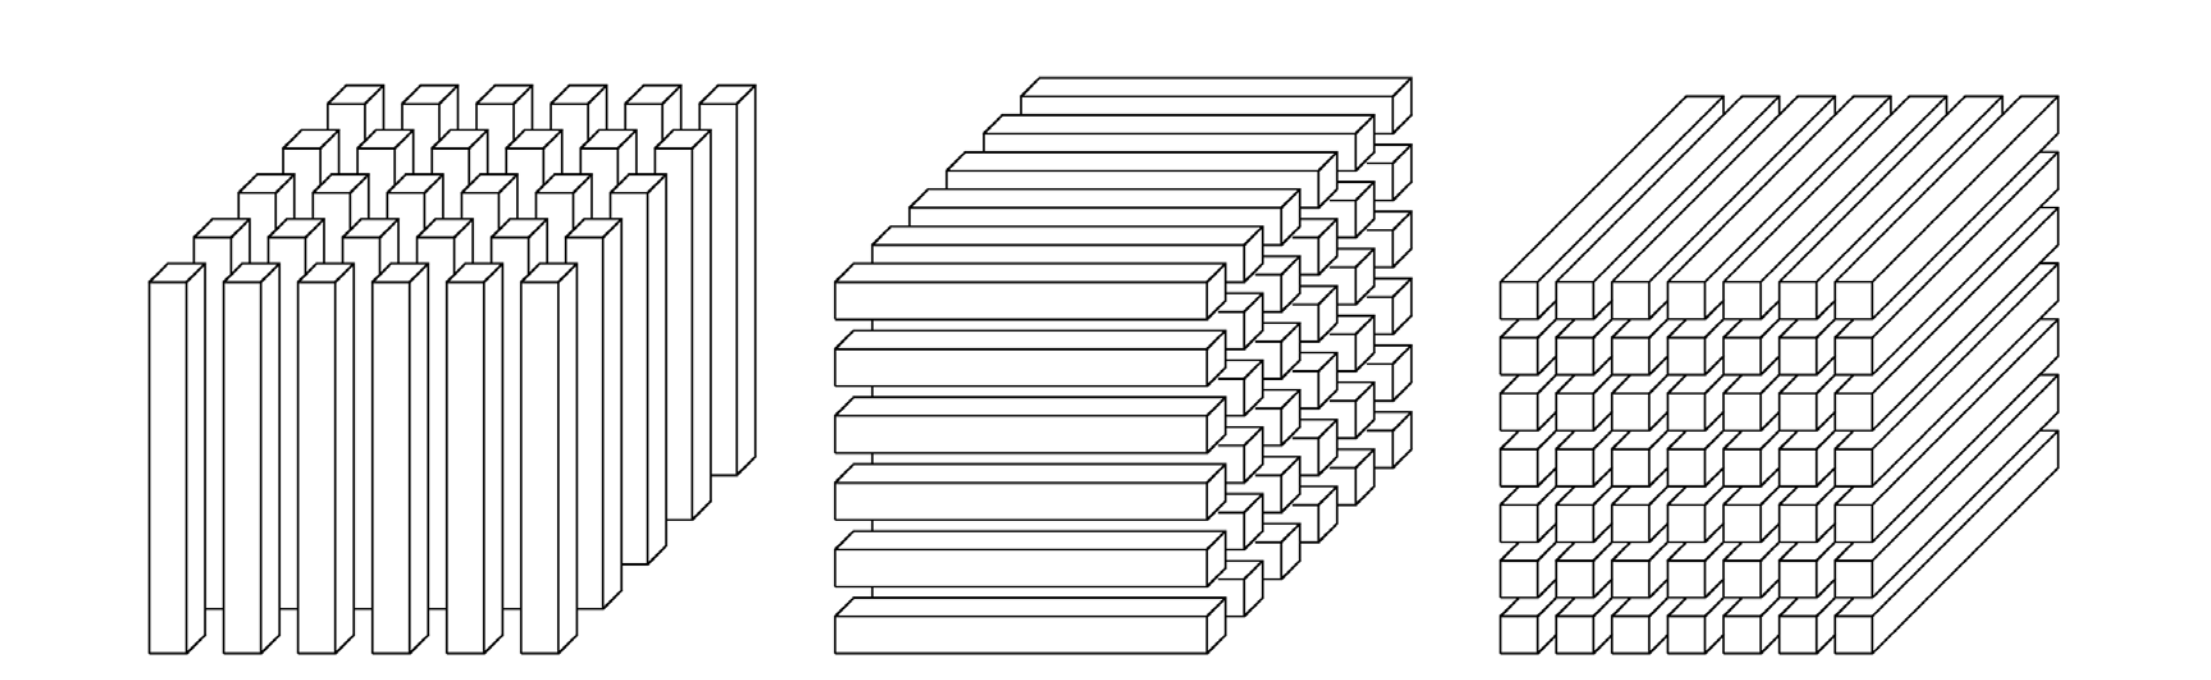
\includegraphics[scale=0.075]{fibers.png}
		\end{center}
		\vspace*{-0.25cm}{\footnotesize Mode-1 (column) fibers: $\T{A}(:,j,k)$, Mode-2 (row) fibers: $\T{A}(i,:,k)$ and Mode-3 (tube) fibers: $\T{A}(i,j,:)$ of a \linebreak 3-dimensional tensor $\T{A}$.}
\end{minipage}\hfill
\begin{minipage}{0.45\linewidth}
	\begin{itemize}
		\item Slices: defined by fixing all indices except two
	\end{itemize}
		\vspace*{-0.525cm}
		\begin{center}
		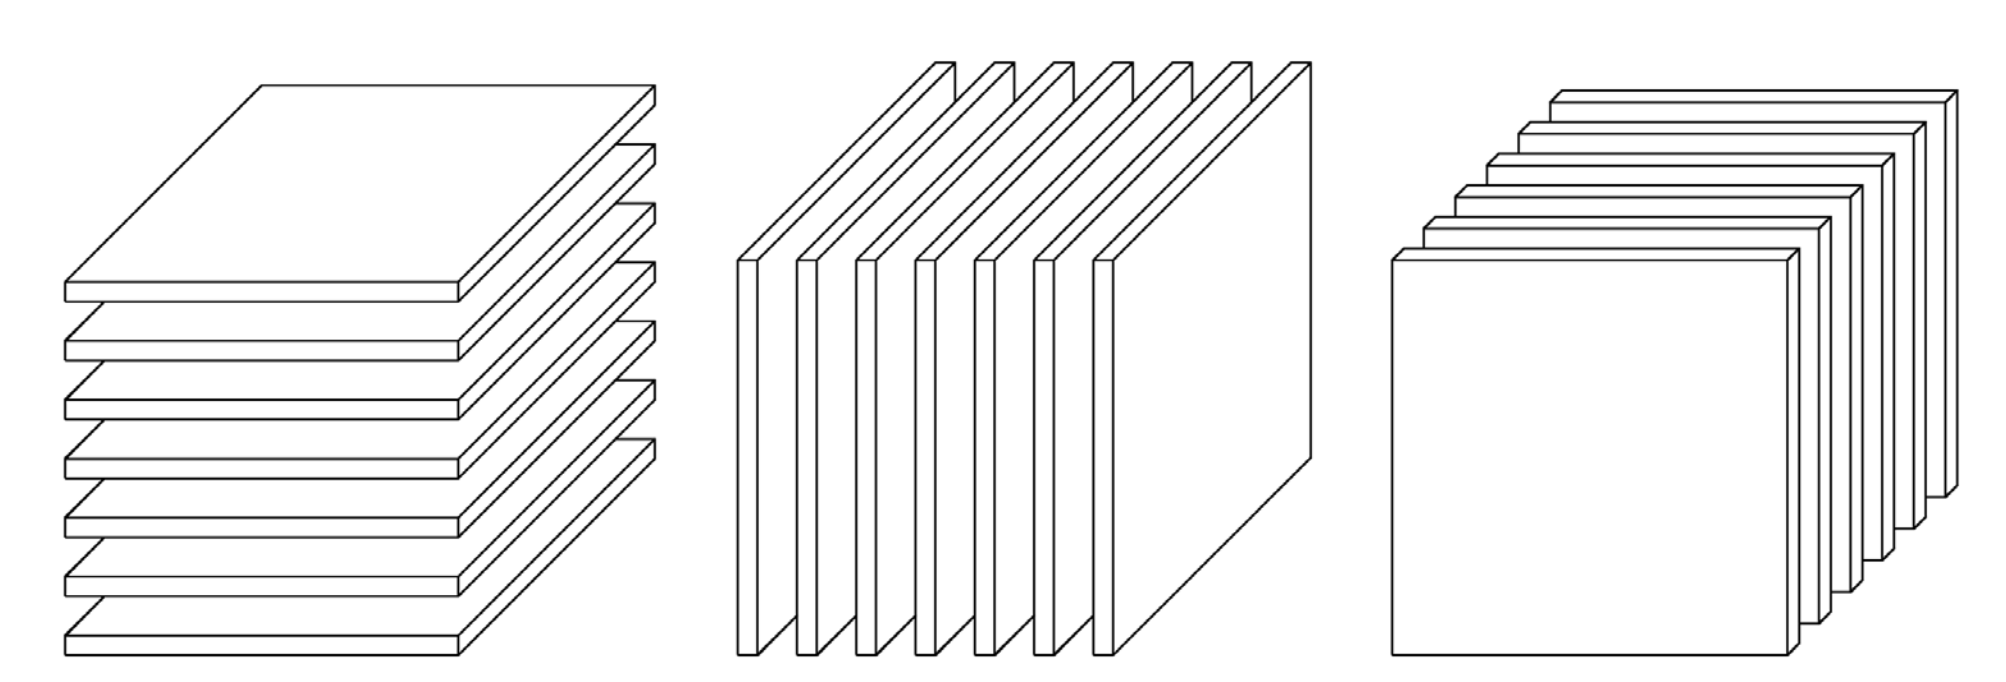
\includegraphics[scale=0.075]{slices.png}	
		\end{center}
		\vspace*{-0.25cm}{\footnotesize Horizontal slices: $\T{A}(i,:,:)$, Lateral slices: $\T{A}(:,j,:)$ and Frontal slices: \linebreak $\T{A}(:,:,k)$ of a 3-dimensional tensor $\T{A}$.}
\end{minipage}
\medskip
\vfill
{\tiny Figures from [Kolda and Bader, 2009].}
\end{frame}

\begin{frame}{Tensor preliminaries}
	\small
	\begin{itemize}
		\item The norm of a tensor $\T{A} \in \mathbb{R}^{n_1\times n_2\times\cdots\times n_d}$ is analogous to the matrix Frobenius norm, and defined as 
		$$||\T{A}|| = \sqrt{\sum_{i_1=1}^{n_1}\sum_{i_2=1}^{n_2}\cdots \sum_{i_d=1}^{n_d}\T{A}^2(i_1,i_2,\cdots,i_d)}$$ 
		\vfill
		\item The inner product of $\T{A},\T{B}  \in \mathbb{R}^{n_1\times n_2\times\cdots \times n_d}$ is 
		$$\langle \T{A},\T{B} \rangle = \sum_{i_1=1}^{n_1}\sum_{i_2=1}^{n_2}\cdots \sum_{i_d=1}^{n_d}\T{A}(i_1,i_2,\cdots,i_d)\T{B}(i_1,i_2,\cdots,i_d)$$
	\end{itemize}
\vfill
		We can note that $\langle \T{A},\T{A} \rangle = ||\T{A}||^2$.
\end{frame}
\begin{frame}{Specific tensors}
	\begin{itemize}
		\item A rank one tensor $\T{A} \in \mathbb{R}^{n_1\times n_2\times\cdots\times n_d}$ can be written as the outer product of $d$ vectors,
			$$\T{A} = u_1 \circ u_2 \circ \cdots \circ u_d$$
			$$\T{A}(i_1,i_2,\cdots,i_d) = u_1(i_1)u_2(i_2)\cdots u_d(i_d) \textnormal{ for all $1\le i_k \le n_k$}$$
		\vfill
		\item A cubical tensor  $\T{A} \in \mathbb{R}^{n_1\times n_2\times\cdots\times n_d}$ has same size in every mode, $$n_1=n_2=\cdots = n_d$$
		\vfill
		\item A supersymmetric (or symmetric) tensor has the same element for any permutation of the indices
		\vfill
		\item A diagonal tensor $\T{A} \in \mathbb{R}^{n_1\times n_2\times\cdots\times n_d}$ has $\T{A}(i_1,i_2,\cdots,i_d) \ne 0 $ only if $i_1=i_2=\cdots=i_d$ 
		
	\end{itemize}
\end{frame}
\begin{frame}{Matricization or Unfolding of a tensor into a matrix}
	\small
	\begin{itemize}
%		\item It reorders the elements of a $d$-dimensional tensor into a matrix
%		\vfill
		\item The mode-$j$ unfolding of $\T{A} \in \mathbb{R}^{n_1\times n_2\times\cdots\times n_d}$ is represented by a matrix $A_{(j)} \in \mathbb{R}^{n_j \times n}$, where $n=n_1n_2\cdots n_{j-1}n_{j+1}\cdots n_d$
		\vfill
		\item Tensor element $\T{A}(i_1,i_2,\cdots,i_d)$ maps to matrix element $A_{(j)}(i_j,k)$, where $k=1+\sum_{\ell=1,\ell\ne j}^{d} (i_\ell-1)N_\ell$ with $N_\ell = \prod_{m=1, m\ne j}^{\ell-1}n_m$
	\end{itemize}
		Example with the frontal slices of $\T{A} \in \mathbb{R}^{4\times 2 \times 3}$:		
{\footnotesize $$\T{A}(:,:,1) = \begin{pmatrix}
1 & 5\\
2 & 6\\
3 & 7\\
4 & 8
\end{pmatrix}, \  \T{A}(:,:,2) = \begin{pmatrix}
9 & 13\\
10 & 14\\
11 & 15\\
12 & 16
\end{pmatrix}, \  \T{A}(:,:,3) = \begin{pmatrix}
17 & 21\\
18 & 22\\
19 & 23\\
20 & 24
\end{pmatrix}$$}
The three mode-$j$ unfoldings are:
{\footnotesize $$A_{(1)} = \begin{pmatrix}
1 & 5 & 9 & 13 & 17 & 21\\
2 & 6 & 10 & 14 & 18 & 22\\
3 & 7 & 11 & 15 & 19 & 23\\
4 & 8 & 12 & 16 & 20 & 24
\end{pmatrix},\  A_{(3)} =\begin{pmatrix}
1 & 2 & 3 & 4 & 5 & 6 & 7 & 8\\
9 & 10 & 11 & 12 & 13 & 14 & 15 & 16\\
17 & 18 & 19 & 20 & 21 & 22 & 23 & 24
\end{pmatrix},$$

$$A_{(2)} = \begin{pmatrix}
1 & 2 & 3 & 4 & 9 & 10 & 11 & 12 & 17 & 18 \quad  19 \quad  20\\
5 & 6 & 7 & 8 & 13 & 14 & 15 & 16 & 21 & 22 \quad  23 \quad  24
\end{pmatrix}$$}	
\end{frame}
\begin{frame}{Assignment 4 -- deadline Oct 10}
	\brown{Question:}Write a program in your preferred programming language to obtain mode-$3$ unfolding of $\T{A}\in \mathbb{R}^{3\times 3\times 3}$. Elements of $\T{A}$ are defined in the following way:
	$$\T{A}(i,j,k) = i+j^2 +k^3 \text{ for } 1\le i,j,k \le 3 \text.$$ 

\vfill
If your preferred language supports $0$-based indexing then you can consider $0\le i,j,k \le 2$.

\vfill

\emph{Submission procedure}: Send your code to my ENS email address (\href{mailto:suraj.kumar@ens-lyon.fr}{suraj.kumar@ens-lyon.fr}) by Oct 10. 
\end{frame}
\begin{frame}{\large Tensor multiplication (contraction) along $j$-mode with a matrix}
\small
The $j$-mode product of $\T{A} \in \mathbb{R}^{n_1\times n_2\times\cdots\times n_d}$ with $U \in \mathbb{R}^{K\times n_j}$ is denoted by  
$\T{A}\times_j U$ and is of size $n_1\times\cdots n_{j-1}\times K \times n_{j+1}\times\cdots\times n_d$.
$$(\T{A}\times_j U)(i_1,\cdots, i_{j-1}, k, i_{j+1}, \cdots i_d) = \sum_{i_j=1}^{n_j} \T{A}(i_1,\cdots,i_d)U(k,i_j)$$
%\vfill
This is also known as tensor-times-matrix (TTM) operation in the $j$th mode.
\vfill
In terms of unfolded tensors:
$$\T{B}=\T{A}\times_j U \Leftrightarrow B_{(j)}= UA_{(j)}$$
\vfill
Some properties of $j$-mode products:
\begin{itemize}
	\item $\T{A} \times_j U \times_k V = \T{A} \times_k V  \times_j U \quad \textnormal{($j\ne k$)}$
	\item $\T{A} \times_j U \times_j V = \T{A} \times_j VU$
\end{itemize}

\end{frame}

\begin{frame}{Matrix products}
	\small
	\begin{itemize}
		\item The Kronecker product of $A\in \mathbb{R}^{m \times n}$ and $B \in \mathbb{R}^{p\times q}$ is $C \in \mathbb{R}^{mp\times nq}$,
		$$C=A\otimes B = \begin{pmatrix}
		A(1,1)B & \cdots & A(1,n)B\\
		\vdots & \ddots & \vdots \\
		A(m,1)B & \cdots & A(m,n)B
		\end{pmatrix}$$
		\vfill
		\item The Khatri-Rao product of $A\in \mathbb{R}^{m \times n}$ and $B \in \mathbb{R}^{p\times n}$ is $C \in \mathbb{R}^{mp\times n}$,
		$$C=A\odot B = \begin{pmatrix}
		A(:,1)\otimes B(:,1) & A(:,2)\otimes B(:,2) & \cdots & A(:,n)\otimes B(:,n)
		\end{pmatrix}$$ 
		\vfill
		\item The Hadamard product of $A\in \mathbb{R}^{m \times n}$ and $B \in \mathbb{R}^{m\times n}$ is $C \in \mathbb{R}^{m\times n}$,
		$$C=A * B = \begin{pmatrix}
		A(1,1)B(1,1) & \cdots & A(1,n)B(1,n)\\
		\vdots & \ddots & \vdots \\
		A(m,1)B(m,1) & \cdots & A(m,n)B(m,n)
		\end{pmatrix}$$
	\end{itemize}
\end{frame}
\begin{frame}{Useful properties of matrix products}
	
	\small
$$(A\otimes B)(C\otimes D) = AC \otimes BD,$$
$$A\odot B \odot C = (A\odot B) \odot C = A \odot (B\odot C)$$
$$(A\odot B)^T(A\odot B) = A^TA * B^TB,$$
$$(A\odot B)^\dagger = ((A^TA) * (B^TB))^\dagger (A\odot B)^T.$$

Here $A^\dagger$ denotes the Moore--Penrose pseudoinverse of $A$.

\vfill

Let $\T{A} \in \mathbb{R}^{n_1\times n_2\times\cdots\times n_d}$  and $U_j \in \mathbb{R}^{m_j\times n_j}$ for $1\le j\le d$. Then,
$$\T{B} = \T{A} \times_1 U_1 \times_2 U_2 \cdots \times_d U_d\qquad\qquad$$
$$\qquad\qquad\qquad\qquad \Leftrightarrow B_{(j)} = U_j A_{(j)}(U_d \otimes \cdots U_{j+1}\otimes U_{j-1}\otimes\cdots\otimes U_1)^T\text.$$
\end{frame}

\section{Tensor decompositions}
\begin{frame}{Table of Contents}		
	\tableofcontents[currentsection,hideallsubsections] % Output the table of contents (all sections on one slide)		
\end{frame}
\begin{frame}{Recap on Singular Value Decomposition (SVD)}
	\small
	\begin{itemize}
		\item It decomposes a matrix $A$ $\in$ $\mathbb{R}^{m \times n}$ to the form $U\Sigma V^T$
		\begin{itemize}
			\item $U$ is an $m\times m$ orthogonal matrix
			\item $V$ is an $n\times n$ orthogonal matrix
			\item $\Sigma$ is an $m\times n$ rectangular diagonal matrix
		\end{itemize}
		\vfill
		\item The diagonal entries $\sigma_i=\Sigma_{ii}$ of $\Sigma$ are called singular values
		\begin{itemize}
			\item $\sigma_i\ge 0$ and $\sigma_1 \ge \sigma_2\ge \cdots \ge \sigma_{\min(m,n)}$
		\end{itemize}
		\vfill
		\item The largest $r$ such that $\sigma_r\ne 0$ is called the rank of the matrix
		\vfill
		\item SVD represents a matrix as the sum of $r$ rank one matrices
	\end{itemize}
	\vfill
	\begin{center}
		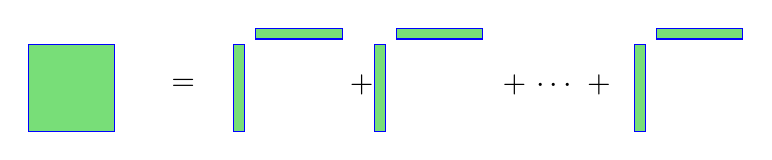
\begin{tikzpicture}[scale=0.275, every node/.style={transform shape}]
		\pgfmathsetmacro{\cubex}{4}
		\pgfmathsetmacro{\cubey}{4}
		\pgfmathsetmacro{\cubez}{4}
		\draw[blue,fill=pastelgreen] (0,0,0) -- ++(-\cubex,0,0) -- ++(0,-\cubey,0) -- ++(\cubex,0,0) -- cycle;
		%%\draw[blue,fill=pastelgreen] (0,0,0) -- ++(0,0,-\cubez) -- ++(0,-\cubey,0) -- ++(0,0,\cubez) -- cycle;
		%%\draw[blue,fill=pastelgreen] (0,0,0) -- ++(-\cubex,0,0) -- ++(0,0,-\cubez) -- ++(\cubex,0,0) -- cycle;
		
		\node[draw=none, text=black, scale=4] at (2,-3,-3) {$=$};
		\pgfmathsetmacro{\smallwidth}{0.5}
		\draw[blue,fill=pastelgreen] (\cubex+2,0,0) -- ++(-\smallwidth,0,0) -- ++(0,-\cubey,0) -- ++(\smallwidth,0,0) -- cycle;
		\draw[blue,fill=pastelgreen] (\cubex+2 +\cubex + 0.5,0.75,0) -- ++(-\cubex,0,0) -- ++(0,-\smallwidth,0) -- ++(\cubex,0,0) -- cycle;
		%%\draw[blue,fill=pastelgreen] (\cubex+2,0.5,0) -- ++(-\smallwidth,0,0) -- ++(0,0,-\cubez) -- ++(\smallwidth,0,0) -- cycle;
		
		\node[draw=none, text=black, scale=4] at (2+\cubex+4.25,-3,-3) {$+$};
		
		\draw[blue,fill=pastelgreen] (\cubex+2.5 + \cubex+2,0,0) -- ++(-\smallwidth,0,0) -- ++(0,-\cubey,0) -- ++(\smallwidth,0,0) -- cycle;
		\draw[blue,fill=pastelgreen] (\cubex+2.5+\cubex+2 +\cubex + 0.5,0.75,0) -- ++(-\cubex,0,0) -- ++(0,-\smallwidth,0) -- ++(\cubex,0,0) -- cycle;
		%%\draw[blue,fill=pastelgreen] (\cubex+2.5+\cubex+2,0.5,0) -- ++(-\smallwidth,0,0) -- ++(0,0,-\cubez) -- ++(\smallwidth,0,0) -- cycle;
		
		\node[draw=none, text=black, scale=4] at (2+\cubex+5 + \cubex+ 4.25, -3,-3) {$+$ $\cdots$ $+$};
		
		\draw[blue,fill=pastelgreen] (12 + \cubex+2.5 + \cubex+2,0,0) -- ++(-\smallwidth,0,0) -- ++(0,-\cubey,0) -- ++(\smallwidth,0,0) -- cycle;
		\draw[blue,fill=pastelgreen] (12+\cubex+2.5+\cubex+2 +\cubex + 0.5,0.75,0) -- ++(-\cubex,0,0) -- ++(0,-\smallwidth,0) -- ++(\cubex,0,0) -- cycle;
		%%\draw[blue,fill=pastelgreen] (12 + \cubex+2.5+\cubex+2,0.5,0) -- ++(-\smallwidth,0,0) -- ++(0,0,-\cubez) -- ++(\smallwidth,0,0) -- cycle;
		\end{tikzpicture}
	\end{center}

\end{frame}



\begin{frame}{Tensor decompositions}
	
	\small
Popular higher-order extension of the matrix SVD:
\begin{itemize}
	\item CANDECOMP/PARAFAC (CP) : proposed by Hitchcock in 1927
	\vfill
	\item Tucker decomposition: proposed by Tucker in 1963
	\vfill
	\item Tensor train decomposition: proposed by Oseledets in 2011, known in quantum chemistry community from a long time with the name of matrix product states
\end{itemize}
\vfill
CP and Tucker decompositions are well suited to work with small and moderate dimension tensors ($d\le 10$). Tensor train is preferred for high dimension tensors.
\end{frame}
\begin{frame}{CP decomposition of $\T{A} \in \mathbb{R}^{n_1\times n_2\times\cdots\times n_d}$}
	\small
	It factorizes a tensor into a sum of rank one tensors.
	\begin{center}
		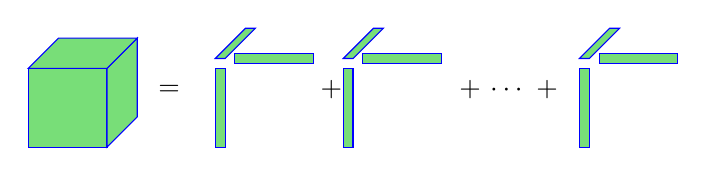
\begin{tikzpicture}[scale=0.25, every node/.style={transform shape}]
		\pgfmathsetmacro{\cubex}{4}
		\pgfmathsetmacro{\cubey}{4}
		\pgfmathsetmacro{\cubez}{4}
		\draw[blue,fill=pastelgreen] (0,0,0) -- ++(-\cubex,0,0) -- ++(0,-\cubey,0) -- ++(\cubex,0,0) -- cycle;
		\draw[blue,fill=pastelgreen] (0,0,0) -- ++(0,0,-\cubez) -- ++(0,-\cubey,0) -- ++(0,0,\cubez) -- cycle;
		\draw[blue,fill=pastelgreen] (0,0,0) -- ++(-\cubex,0,0) -- ++(0,0,-\cubez) -- ++(\cubex,0,0) -- cycle;
		
		\node[draw=none, text=black, scale=4] at (2,-2.25,-3) {$=$};
		\pgfmathsetmacro{\smallwidth}{0.5}
		\draw[blue,fill=pastelgreen] (\cubex+2,0,0) -- ++(-\smallwidth,0,0) -- ++(0,-\cubey,0) -- ++(\smallwidth,0,0) -- cycle;
		\draw[blue,fill=pastelgreen] (\cubex+2 +\cubex + 0.5,0.75,0) -- ++(-\cubex,0,0) -- ++(0,-\smallwidth,0) -- ++(\cubex,0,0) -- cycle;
		\draw[blue,fill=pastelgreen] (\cubex+2,0.5,0) -- ++(-\smallwidth,0,0) -- ++(0,0,-\cubez) -- ++(\smallwidth,0,0) -- cycle;
		
		\node[draw=none, text=black, scale=4] at (2+\cubex+4.25,-2.25,-3) {$+$};
		
		\draw[blue,fill=pastelgreen] (\cubex+2.5 + \cubex+2,0,0) -- ++(-\smallwidth,0,0) -- ++(0,-\cubey,0) -- ++(\smallwidth,0,0) -- cycle;
		\draw[blue,fill=pastelgreen] (\cubex+2.5+\cubex+2 +\cubex + 0.5,0.75,0) -- ++(-\cubex,0,0) -- ++(0,-\smallwidth,0) -- ++(\cubex,0,0) -- cycle;
		\draw[blue,fill=pastelgreen] (\cubex+2.5+\cubex+2,0.5,0) -- ++(-\smallwidth,0,0) -- ++(0,0,-\cubez) -- ++(\smallwidth,0,0) -- cycle;
		
		\node[draw=none, text=black, scale=4] at (2+\cubex+5 + \cubex+ 4.25, -2.25,-3) {$+$ $\cdots$ $+$};
		
		\draw[blue,fill=pastelgreen] (12 + \cubex+2.5 + \cubex+2,0,0) -- ++(-\smallwidth,0,0) -- ++(0,-\cubey,0) -- ++(\smallwidth,0,0) -- cycle;
		\draw[blue,fill=pastelgreen] (12+\cubex+2.5+\cubex+2 +\cubex + 0.5,0.75,0) -- ++(-\cubex,0,0) -- ++(0,-\smallwidth,0) -- ++(\cubex,0,0) -- cycle;
		\draw[blue,fill=pastelgreen] (12 + \cubex+2.5+\cubex+2,0.5,0) -- ++(-\smallwidth,0,0) -- ++(0,0,-\cubez) -- ++(\smallwidth,0,0) -- cycle;
		\end{tikzpicture}
	\end{center}
		\vspace*{-0.15cm}\centering{\footnotesize CP decomposition of a $3$-dimensional tensor.}
	\vfill
	{\footnotesize\vspace*{-0.1cm}$$\T{A}=\sum_{\alpha=1}^{r} U_1 (:,\alpha) \circ U_2(:,\alpha)\circ\cdots \circ U_d(:,\alpha)$$
	$$\T{A}(i_1,\cdots,i_d) = \sum_{\alpha=1}^{r} U_1(i_1,\alpha) U_2(i_2,\alpha)\cdots U_d(i_d,\alpha)$$}
	\vfill
	The minimum $r$ required to express $\T{A}$ is called the rank of $\T{A}$. The matrices $U_j \in \mathbb{R}^{n_j\times r}$ for $1\le j \le d$ are called factor matrices.$\qquad\qquad\qquad\qquad\qquad$
	\vfill
	\begin{itemize}
		\item ({\color{green}+}) The number of entries in a CP decomposition of {\footnotesize $\T{A} = \mathcal{O}((n_1+\cdots + n_d)r)$}
%		\item ({\color{green}+}) For $n_1=n_2=\cdots n_d=n$, the number of entries = $\mathcal{O}(nrd)$
		\item ({\color{red}-}) Determining the minimum value of $r$ is an NP-complete problem
		\item ({\color{red}-}) No robust algorithms to compute this representation
	\end{itemize}
\end{frame}


\begin{frame}{Tucker decomposition of $\T{A} \in \mathbb{R}^{n_1\times n_2\times\cdots\times n_d}$}
	
	\small
	It represents a tensor with $d$ matrices (usually orthogonal) and a small core tensor.
	\begin{center}
		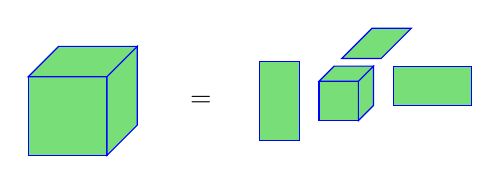
\begin{tikzpicture}[scale=0.25, every node/.style={transform shape}]
		\pgfmathsetmacro{\cubex}{4}
		\pgfmathsetmacro{\cubey}{4}
		\pgfmathsetmacro{\cubez}{4}
		\draw[blue,fill=pastelgreen] (-12,1,\cubez-2) -- ++(-\cubex,0,0) -- ++(0,-\cubey,0) -- ++(\cubex,0,0) -- cycle;
		\draw[blue,fill=pastelgreen] (-12,1,\cubez-2) -- ++(0,0,-\cubez) -- ++(0,-\cubey,0) -- ++(0,0,\cubez) -- cycle;
		\draw[blue,fill=pastelgreen] (-12,1,\cubez-2) -- ++(-\cubex,0,0) -- ++(0,0,-\cubez) -- ++(\cubex,0,0) -- cycle;
		\node[draw=none, text=black, scale=4] at (-8,-1,0) {$=$};
		
		\pgfmathsetmacro{\cubex}{2}
		\pgfmathsetmacro{\cubey}{2}
		\pgfmathsetmacro{\cubez}{2}
		\draw[blue,fill=pastelgreen] (0,0,0) -- ++(-\cubex,0,0) -- ++(0,-\cubey,0) -- ++(\cubex,0,0) -- cycle;
		\draw[blue,fill=pastelgreen] (0,0,0) -- ++(0,0,-\cubez) -- ++(0,-\cubey,0) -- ++(0,0,\cubez) -- cycle;
		\draw[blue,fill=pastelgreen] (0,0,0) -- ++(-\cubex,0,0) -- ++(0,0,-\cubez) -- ++(\cubex,0,0) -- cycle;
		
		\draw[blue,fill=pastelgreen] (-\cubex-1,1,0) -- ++(-\cubex,0,0) -- ++(0,-\cubey-2,0) -- ++(\cubex,0,0) -- cycle;
		\draw[blue,fill=pastelgreen] (\cubex+2+1,0,-\cubey) -- ++(-\cubex-2,0,0) -- ++(0,-\cubey,0) -- ++(\cubex+2,0,0) -- cycle;
		
		\draw[blue,fill=pastelgreen] (0,0,-\cubez-1) -- ++(-\cubex,0,0) -- ++(0,0,-\cubez-2) -- ++(\cubex,0,0) -- cycle;
		\end{tikzpicture}
	\end{center}
			\vspace*{-0.15cm}\centering{\footnotesize Tucker decomposition of a $3$-dimensional tensor.}
			\vfill
			{\footnotesize\vspace*{-0.1cm}$$\T{A} = \T{G} \times_1 U_1 \cdots \times_d U_d$$
			$$\T{A}(i_1,\cdots,i_d) = \sum_{\alpha_1=1}^{r_1}\cdots\sum_{\alpha_d=1}^{r_d} \T{G}(\alpha_1,\cdots,\alpha_d)U_1(i_1,\alpha_1)\cdots U_d(i_d, \alpha_d)$$}
			\vfill
			Here $r_j$ for $1\le j\le d$ denote a set of ranks. Matrices $U_j \in \mathbb{R}^{n_j\times r_j}$ for $1\le j \le d$ are called factor matrices. The tensor $\T{G}\in \mathbb{R}^{r_1\times r_2\times\cdots\times r_d}$ is called the core tensor.
			\vfill 
	\begin{itemize}
		\item ({\color{green}+}) SVD based stable algorithms to compute this decomposition
		\item ({\color{red}-}) The number of entries = $\mathcal{O}(n_1r_1 + \cdots + n_dr_d+ \prod_{j=1}^{d}r_j)$
%		\item ({\color{red}-}) For $n_1=n_2=\cdots n_d=n$ and $r_1=r_2=\cdots =r_d=r$, the number of entries = $\mathcal{O}(ndr+r^d)$
	\end{itemize}	
\end{frame}

%------------------------------------------------
\begin{frame}{\large Tensor Train (TT) decomposition: Product of matrices view}
	
	\small
	\begin{itemize}
		\item A $d$-dimensional tensor is represented with $2$ matrices and $d$-$2$ $3$-dimensional tensors.
	\end{itemize}
	\begin{figure}
		\begin{center}	
			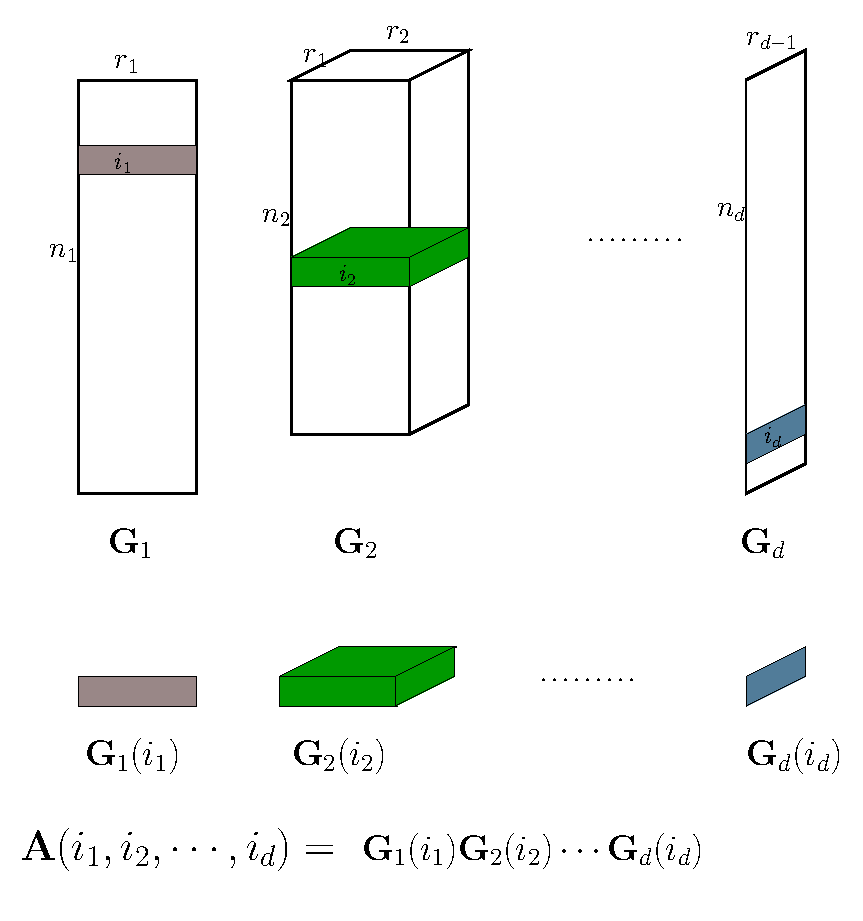
\includegraphics[scale=0.325]{./ttentry.eps}
		\end{center}
	\end{figure}
	\noindent An entry of $\T{A}$ $\in$ $\mathbb{R}^{n_1 \times \cdots \times n_d}$ is computed by multiplying corresponding matrix (or row/column) of each matrix/tensor.
\end{frame}

\begin{frame}{Tensor Train decomposition}
	
	\begin{block}{}
		$\T{A}$ $\in$ $\mathbb{R}^{n_1 \times \cdots \times n_d}$ is represented with cores $\T{G}_k$$\in$ $\mathbb{R}^{r_{k-1}\times n_k\times r_k}$, $k$=$1,2,\cdots d$, $r_0$=$r_d$=$1$ and its elements satisfy the following expression:
		{\small\begin{align*}
			\T{A}(i_1,\cdots ,i_d) 
			&= \sum_{\alpha_0 = 1}^{r_0} \cdots \sum_{\alpha_d = 1}^{r_d} \T{G}_1(\alpha_0, i_1, \alpha_1) \cdots \T{G}_d(\alpha_{d-1}, i_d, \alpha_d)\\
			&= \sum_{\alpha_1 = 1}^{r_1} \cdots \sum_{\alpha_{d-1} = 1}^{r_{d-1}} \T{G}_1(1, i_1, \alpha_1) \cdots \T{G}_d(\alpha_{d-1}, i_d, 1)
			\end{align*}}
		\begin{center}
			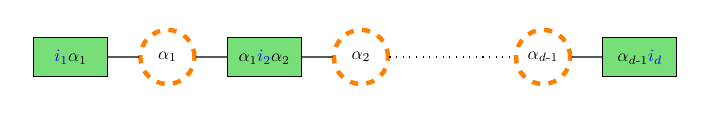
\begin{tikzpicture}[scale=0.625, every node/.style={transform shape}]
			\tikzstyle{taskc}=[circle, draw=orange, minimum size=11mm, fill=none, dashed, ultra thick]
			\tikzstyle{taskr}=[draw=black, minimum height=8mm, minimum width=15mm, anchor=south west, fill=pastelgreen, text=black]
			
			\node(t1) at (0,0) {};
			\node [above right=0cm and 0cm of t1.mid,taskr](T1) {$\textcolor{blue}{i_1}\alpha_1$};
			\node [above right=0cm and 0.8cm of T1.south east, taskc](C1) {$\alpha_1$};
			\node [above right=0cm and 0.8cm of C1.south east, taskr](T2) {$\alpha_1\textcolor{blue}{i_2}\alpha_2$};
			\node [above right=0cm and 0.8cm of T2.south east, taskc](C2) {$\alpha_2$};
			
			\node [above right=0cm and 4.5cm of T2.south east, taskc](Cd) {$\alpha_{d\text{-}1}$};
			\node [above right=0cm and 0.8cm of Cd.south east, taskr](Td) {$\alpha_{d\text{-}1}\textcolor{blue}{i_d}$};
			\draw (T1.east)--(C1.west);
			\draw (C1.east)--(T2.west);
			\draw (T2.east)--(C2.west);
			\draw [dotted] (C2.east)--(Cd.west);
			\draw (Cd.east)--(Td.west);
			\path (-0.1, -0.4) -- (2.5, -0.4); 
			%%\path (-0.1, -0.8) -- (2.5, -0.8); 
			\end{tikzpicture}
		\end{center}
	\end{block}
The ranks $r_k$ are called TT-ranks.
	\begin{itemize}
		\item The number of entries in this decomposition = $\mathcal{O}(n_1r_1 + n_2r_1r_2 + n_3r_2r_3+\cdots + n_{d-1}r_{d-2}r_{d-1} + n_dr_{d-1})$
%		\item For $n_1=n_2=\cdots=n_d=n$ and $r_1=r_2=\cdots=r_{d-1}=r$, the number of entries = $\mathcal{O}(ndr^2)$
	\end{itemize}
\end{frame}

\end{document} 